\documentclass{article}
\usepackage[margin=2cm]{geometry}

\usepackage{amsmath, amssymb, amsthm}
\usepackage{fancyhdr}
\usepackage{pgfplots}

\begin{document}

\begin{figure}
\centering
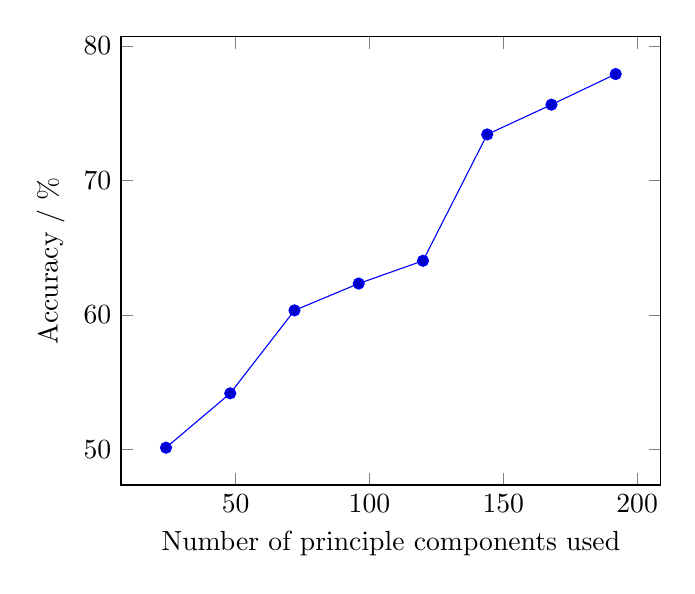
\begin{tikzpicture}
  \begin{axis}[
      xlabel={Number of principle components used},
      ylabel={Accuracy / \%}]
    ]
      \addplot coordinates {
        (24, 50.14)
        (48, 54.177)
        (72, 60.341)
        (96, 62.334)
        (120, 64.027)
        (144, 73.415)
        (168, 75.628)
        (192, 77.9)
      };
  \end{axis}
\end{tikzpicture}
\caption{Using PCA to perform dimension reduction is not always a good idea. }
\end{figure}

\begin{figure}
\label{tabAcc}
\centering
\begin{tabular}{|c|c|}
  \hline
  \textbf{Method} & \textbf{Accuracy}\\
  \hline
  Random & 10.0\%\\
  Raw pixels & 37.3\%\\
  K-means + all PCs & 77.9\%\\
  K-means + 0.99 variance & 50.0\%\\
  Sparse K-means & 83.0\%\\
  \hline
\end{tabular}
\end{figure}

\begin{figure}
\label{figSparseKM}
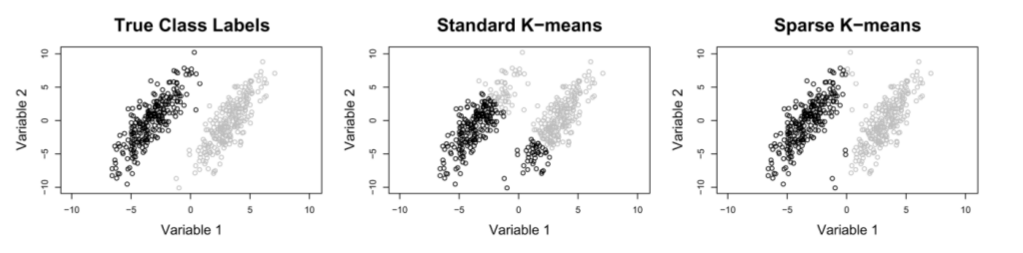
\includegraphics[width=\columnwidth]{./sparse.png}
\caption{Sparse K-means helps us perform feature selection}
\end{figure}
Figure \ref{tabAcc} shows the accuracy performed on CIFAR-10 from (1) randomly choosing a class (2) raw pixels fed into an SVM (3) the K-means algorithm described (4) K-means with PCA on patches (5) sparse K-means to reduce dimensionality.

Running an SVM against raw pixels shows us that raw pixels do not make for a good feature representation for image classification.

Running PCA on image patches also sacrifices a large amount of accuracy. If we were to run PCA on the data in Figure \ref{figSparseKM} we would not be able to get good clusters on the new space. This is reflected in the accuracy drop from using PCA based on the total variance of the data.

\end{document}
